\chapter{Key Distribution Scheme}\label{chp3:file-sync}
This chapter will first introduce the application that makes the key distribution scheme possible over \gls{NDN}.
The application, \gls{FSM}, is designed to be applicable to any other distribution of files over \gls{NDN}.
The key distribution scheme and key revocation I use in the~\autoref{sensor-application} will be presented.

\section{File Synchronization Module}\label{file-sync}
The \gls{FSM} is built upon ChronoSync, which is explained in~\autoref{apx:chronosync}.
The goal for the \gls{FSM} is to distribute \gls{data} to a large group of nodes.
Each node wants to verify that the distributed \gls{data} originate from the \gls{publisher}.
Each node always wants to have the newest version of the \gls{data}. 
One example where \gls{FSM} is applicable is when we want to distribute a list of public keys within a domain.
Let us say there is a list owner, e.g. a \gls{TTP} that could be a university like the \gls{ntnu}.
\gls{ntnu} wants to distribute to a large set of nodes, i.e. each student and employee at \gls{ntnu}.
Every node wants to have every public key in \gls{ntnu}s domain up-to-date.
When the list of public keys gets updated, caused by for instance a key revocation or a key initialization, every node should immediately synchronize with the updated list.

There can be two types of roles in the \gls{FSM}. 
\begin{enumerate}
	\item Distributor
	\item Subscriber
\end{enumerate}
Distributors are list-owners and have read-write access.
Subscribers only have read access.
A node can be both a distributor and a subscriber, and there can be several distributors that are equal, i.e. several owners of the list.
However, there is one root distributor (i.e. the true owner) that should be able to delegate write access to other nodes that should act as a distributor. 
The capabilities is distributed to all nodes and signed by the root distributor.
These capabilities is needed so that every node can verify the integrity and authenticity of the distributed list.
If confidentiality is required, it can be achieved by symmetric encryption, and key exchange in the subscription protocol, i.e. using asymmetric encryption.
However this becomes quite complicated concerning possible key leakage and redistribution of a new symmetric key when the number of subscribers is high. 
In the case of public keys list, the data would not have to be confidential, but rather rely on integrity and authenticity.

In~\autoref{fig:ndn-sync} the subscribers (\texttt{a}, \texttt{b} and \texttt{c}) wants to subscribe to the distributors' (\texttt{d}) list of public keys.
In order to achieve this goal, the following actions should occur.
\begin{enumerate}
	\item \texttt{d} announces that it wants to distribute a list to the network by registering the synchronization group prefix. 
	\item \texttt{a}, \texttt{b} and \texttt{c} ask for subscription to this list, and somehow authenticates them selves to \texttt{d} if confidentiality is required.
	\item \texttt{d} approves those who should be approved, and returns a symmetric synchronization key. 
	This step is only done if confidentiality is required.
	\item \texttt{a}, \texttt{b} and \texttt{c} now knows that they are a part of the synchronization and have read access. They expresses a \texttt{Sync} \gls{interest} with their state, receiving \texttt{Sync} \gls{data} whenever \texttt{d} has announced a newer state.
\end{enumerate}

\begin{figure}[ht]
  \centering
  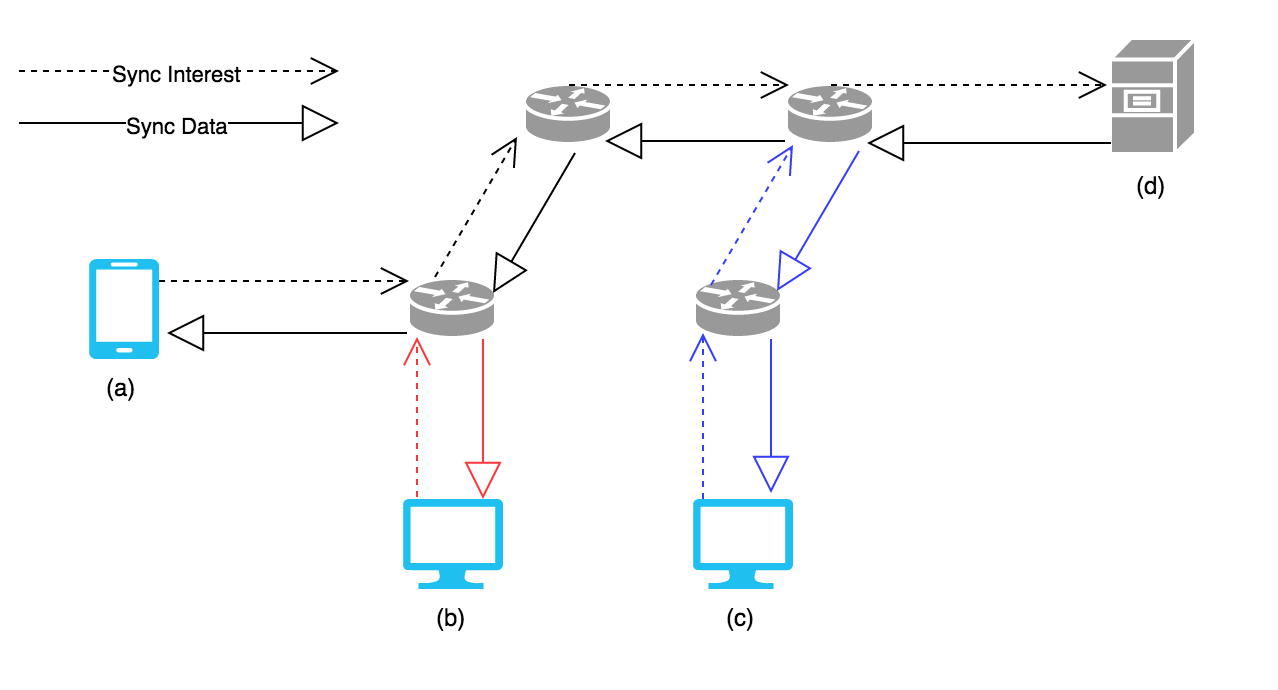
\includegraphics[width=1\textwidth]{ndn-sync.png}
  \caption[File Synchronization in NDN]{File Synchronization in NDN.}
  \label{fig:ndn-sync}
\end{figure}

\section{Key Distribution}\label{key-distribution}
In traditional \gls{PKI}, each public key is signed by a certificate authority and the generated certificate is sent as a response over a secure channel then validated by the the client.
I want to make the certificate authority obsolete by distributing every \gls{ID} with the \gls{PKG} acting as a \gls{kdc}, as explained in the above section.
In~\autoref{fig:pkg_sync} we see that the \gls{PKG} multicasts the \gls{ID} list to all devices that have joined the trust domain.
Each device can verify the integrity and authenticity of the sync state \gls{data} and validate that the \gls{ID} list surely originates from its own \gls{PKG}, i.e. the distributor.
\begin{figure}[ht]
  \centering
  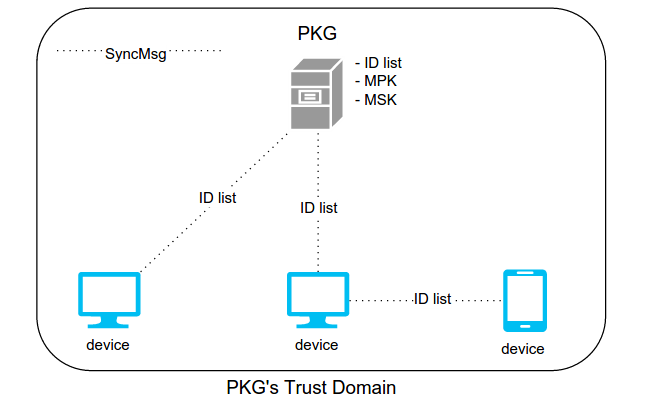
\includegraphics[width=1\textwidth]{pkg_sync.png}
  \caption[File Synchronization Module]{FSM with tree devices (subscribers) and a PKG (distributor).}
  \label{fig:pkg_sync}
\end{figure}


\section{Key Revocation}
Key revocation in systems are studied well in traditional \gls{PKI}.
However, few alternatives to revocation schemes in \gls{IBE} \gls{PKI} have been proposed.
One suggestion is to allocate secret keys with the \gls{ID} combined with some sort of date, e.g. month-year or just year~\cite[section 1.1.1]{DBLP:conf/crypto/BonehF01}. 
In this alternative a user has to renew its secret key each time the date changes, i.e. either the month or the year depending on the date format.
The problem with this revocation solution is that it can be cumbersome for the \gls{PKG}.
Boldyreva et al. proposes a revocation scheme~\cite{DBLP:journals/iacr/BoldyrevaGK12} based on efficient key-update, which makes the workload for the \gls{PKG} a lot easier. 
This scheme was only proven secure in the selective-ID setting where adversaries can attack an \gls{ID} given they choose which one at the beginning of the game.
The work done by Beno\^{i}t Libert and Damien Vergnaud in~\cite{DBLP:conf/ctrsa/LibertV09} solves this problem. 
However, efficiently delegating both the key generation and revocation functionalities was a problem left open.
Jae Hong Seo and Keita Emura solves this in~\cite{DBLP:journals/iacr/SeoE13a}.

Basically there exist two use cases where we want to renew a \gls{SK}: 
\begin{enumerate}
  \item when the \gls{SK} is compromised.
  \item when the renewal period has expired.
\end{enumerate}
If a key is compromised, we want to revoke the key immediately letting everybody know that this specific \gls{ID} has been revoked. 
One problem with key revocation is that there is no way of revoking this key, and thus the \gls{ID} has to be changed and distributed. 
However, a partially revocation can be sufficient in some networks. 
By partially, I do not mean revoking the \gls{SK}, but rather only distributing the new \gls{ID} to every node in the trust domain.
In short, the compromised key should be removed from a distributed ID-list and the list containing only valid \gls{ID}s should be disseminated.
With the \gls{FSM}, the list is distributed automatically when updated, and only a \gls{DoS} attack together with a compromised key would make the system vulnerable. 

Some periodic renewal might be necessary in many systems because it is not always known that a key has been compromised.
If such an \gls{ID} structure is applied, the key distribution should only contain the base key of each device. 